% =============================================================================
% Chapter 7: System Architecture and Implementation
% Pit-Viper-Inspired Infrared-Thermal and Visual Sensor Fusion
% for Nocturnal UAV Navigation
% =============================================================================

\selectlanguage{hebrew}

\section{ארכיטקטורת מערכת ומימוש}
\label{sec:ch07_system_architecture}

\subsection{סקירת המערכת הכוללת}
\label{sec:ch07_overview}

בפרק זה אנו מציגים את הארכיטקטורה המלאה של מערכת המיזוג התרמי-חזותי שפותחה במסגרת מחקר זה. המערכת, הקרויה \en{ThermalVisionFusion} (בקיצור \en{TVF}), מהווה מימוש שלם של העקרונות הביולוגיים שנדונו בפרקים הקודמים, תוך התאמה לדרישות ההפעלה בזמן אמת על פלטפורמת רחפן מוגבלת משאבים. הארכיטקטורה מבוססת על שלוש שכבות עיקריות: שכבת רכישת הנתונים, שכבת העיבוד והמיזוג, ושכבת הניווט והבקרה. כל שכבה כוללת רכיבי חומרה ותוכנה ייעודיים המתואמים זה לזה באמצעות ממשקים מוגדרים היטב.

המערכת תוכננה מתוך ראייה מערכתית כוללת, תוך התחשבות באילוצי ההספק, המשקל והזמן-אמת האופייניים לרחפנים קטנים (\en{Micro Aerial Vehicles}, \en{MAVs}). בחירת הרכיבים נעשתה על בסיס ניתוח עלות-תועלת קפדני, תוך איזון בין דיוק לביצועים. המערכת מבוססת על לוח \en{NVIDIA Jetson Orin NX} כמעבד המרכזי, המספק 70 \en{TOPS} של ביצועי \en{AI} בהספק של 25 ואט בלבד. בחירה זו מאפשרת הרצת מודלי רשתות עצביות מורכבות בזמן אמת, תוך שמירה על חיי סוללה סבירים למשימות ניווט לילי של 30-45 דקות.

הארכיטקטורה כוללת שלושה חיישנים עיקריים: מצלמת \en{RGB} מסוג \en{FLIR Blackfly S BFS-U3-51S5C} ברזולוציית 5.1 מגה-פיקסל וקצב של 30 פריימים לשנייה, מצלמת תרמית מסוג \en{FLIR Boson 640} ברזולוציית 640x512 פיקסלים וקצב של 60 הרץ, ויחידת \en{IMU} מסוג \en{InvenSense ICM-20948} בתדר 400 הרץ. כל החיישנים מכוילים מרחבית וזמנית באמצעות שיטת הכיול המתוארת בסעיף \ref{sec:ch07_calibration}. הנתונים מהחיישנים השונים מסונכרנים באמצעות חותמות זמן חומרתיות המבוססות על פרוטוקול \en{PTP (Precision Time Protocol)}.

\subsection{ארכיטקטורת חומרה}
\label{sec:ch07_hardware}

פלטפורמת הרחפן מבוססת על שלדת \en{DJI M300 RTK} שעברה התאמה אישית לנשיאת מערך החיישנים. משקל ההמראה הכולל הוא 6.3 ק"ג, מתוכם 1.2 ק"ג מיועדים למערכת החיישנים והמחשוב. צריכת ההספק הכוללת של מערכת החיישנים והעיבוד היא 45 ואט, המאפשרת זמן טיסה של 35 דקות בתנאי לילה. טבלה \ref{tab:ch07_hardware_specs} מציגה את מפרט הרכיבים העיקריים.

\begin{table}[htbp]
\centering
\caption{מפרט רכיבי החומרה העיקריים של מערכת \en{TVF}.}
\label{tab:ch07_hardware_specs}
\adjustbox{max width=\columnwidth}{%
\begin{tabular}{@{}lccc@{}}
\toprule
\textbf{רכיב} & \textbf{דגם} & \textbf{מפרט} & \textbf{הספק [ואט]} \\
\midrule
מעבד ראשי & \en{Jetson Orin NX} & 8 ליבות \en{Cortex-A78AE}, 1024 ליבות \en{GPU} & 25 \\
מצלמת \en{RGB} & \en{Blackfly S BFS-U3-51S5C} & 5.1 MP, 30 \en{fps}, \en{CMOS} $1/2.5"$ & 3.2 \\
מצלמה תרמית & \en{FLIR Boson 640} & 640x512, 60 \en{fps}, 7.5-13.5 $\mu$m & 1.8 \\
יחידת \en{IMU} & \en{ICM-20948} & 9-ציר, 400 \en{Hz}, $\pm$16g & 0.15 \\
מודול \en{GPS} & \en{u-blox F9P} & \en{RTK}, 10 \en{Hz}, 2.5 \en{cm} דיוק & 0.5 \\
סוללה & \en{TB60} & 6000 \en{mAh}, 6S \en{LiPo} & : \\
\bottomrule
\end{tabular}%
}
\end{table}

החיישנים מותקנים על גבי פלטפורמה מיוצבת בתלת-ציר (\en{3-axis gimbal}) המבטלת רעידות בתדר גבוה ומאפשרת כיוון מדויק של שדות הראייה. המרחק בין מרכזי העדשות של המצלמה החזותית והתרמית הוא 4.5 ס"מ, מה שמאפשר רישום גיאומטרי מדויק עם מקבילית מינימלית. כיול משותף של כל החיישנים בוצע באמצעות שיטת הכיול המתוארת בסעיף \ref{sec:ch07_calibration}, תוך השגת דיוק רישום של 0.8 פיקסלים בין המצלמות.

\subsection{כיול חיישנים משותף}
\label{sec:ch07_calibration}

כיול משותף של מערך החיישנים הרב-מודאלי הוא תנאי הכרחי למיזוג נתונים אפקטיבי. תהליך הכיול כולל שלושה שלבים עיקריים: כיול אינטרינזי של כל מצלמה בנפרד, כיול אקסטרינזי בין המצלמות, וכיול זמני בין כל החיישנים. הכיול האינטרינזי מבוסס על שיטת \en{Zhang} תוך שימוש בלוח שחמט סטנדרטי הנראה גם בתחום התרמי בזכות ציפוי מיוחד.

מודל המצלמה עבור כל חיישן מבוסס על מודל החור (\en{pinhole model}) עם תיקון עיוותים רדיאליים ומשיקיים:

\begin{equation}
\left[u \\ v \\ 1\right] = \mathbf{K} \cdot \left[\mathbf{R},\; \mathbf{t}\right] \cdot \left[X \\ Y \\ Z \\ 1\right], \quad \mathbf{K} = \left[f_x,\; 0,\; c_x \\ 0,\; f_y,\; c_y \\ 0,\; 0,\; 1\right]
\label{eq:ch07_pinhole}
\end{equation}

כאשר $\mathbf{K}$ היא מטריצת הכיול האינטרינזי, $f_x, f_y$ הם אורכי המוקד, $c_x, c_y$ הן קואורדינטות מרכז התמונה, ו-$\mathbf{R}, \mathbf{t}$ הם פרמטרי הסיבוב והתרגום האקסטרינזיים. מודל העיוות הרדיאלי מתואר על ידי:

\begin{equation}
\left[u_d \\ v_d\right] = (1 + k_1 r^2 + k_2 r^4 + k_3 r^6) \left[u \\ v\right] + \left[2p_1 uv + $p_2(r^2 + 2u^2)$ \\ $p_1(r^2 + 2v^2)$ + 2p_2 uv\right]
\label{eq:ch07_distortion}
\end{equation}

כאשר $r^2 = u^2 + v^2$, $k_1, k_2, k_3$ הם מקדמי העיוות הרדיאלי, ו-$p_1, p_2$ הם מקדמי העיוות המשיקי. הכיול בוצע באמצעות 50 תמונות של לוח השחמט מזוויות שונות, תוך שימוש באלגוריתם \en{Levenberg-Marquardt} למזעור שגיאת ההיטל מחדש. שגיאת הכיול הממוצעת היא 0.12 פיקסלים עבור המצלמה החזותית ו-0.28 פיקסלים עבור המצלמה התרמית.

הכיול האקסטרינזי בין המצלמות מבוסס על התאמת נקודות ייחוס הנראות בשני התחומים הספקטרליים. לשם כך פותח לוח כיול ייעודי המשלב דפוס שחמט סטנדרטי עם מקורות חום נקודתיים (\en{LEDs} תרמיים) הנראים בבירור בתמונה התרמית. הטרנספורמציה בין מערכות הקואורדינטות מתוארת על ידי:

\begin{equation}
\mathbf{T}_{\text{ir}}^{\text{vis}} = \left[\mathbf{R}_{\text{ir}}^{\text{vis}},\; \mathbf{t}_{\text{ir}}^{\text{vis}} \\ \mathbf{0}^T,\; 1\right] \in SE(3)
\label{eq:ch07_extrinsic}
\end{equation}

הכיול הזמני מבוסס על סנכרון חותמות הזמן של כל החיישנים באמצעות פרוטוקול \en{PTP (IEEE 1588)}. הפרש הזמן בין החיישנים נשמר מתחת ל-100 מיקרו-שניות, מה שמבטיח התאמה זמנית מדויקת בין הנתונים השונים. בנוסף, מבוצע תיקון דינמי של הפרשי הזמן באמצעות אלגוריתם \en{correlation-based synchronization} המתואר בסעיף \ref{sec:ch07_sync}.

\subsection{פיפטת עיבוד תמונה}
\label{sec:ch07_pipeline}

פיפטת עיבוד התמונה של המערכת כוללת חמישה שלבים עיקריים: רכישה, עיבוד מקדים, רישום, מיזוג, וניתוח. כל שלב מתוכנן לפעול בזמן אמת תוך עמידה במגבלות ההשהיה של מערכת הניווט. איור \ref{fig:sensor_architecture} מציג את הארכיטקטורה המלאה של פיפטת העיבוד.

\begin{figure*}[htbp]
\centering
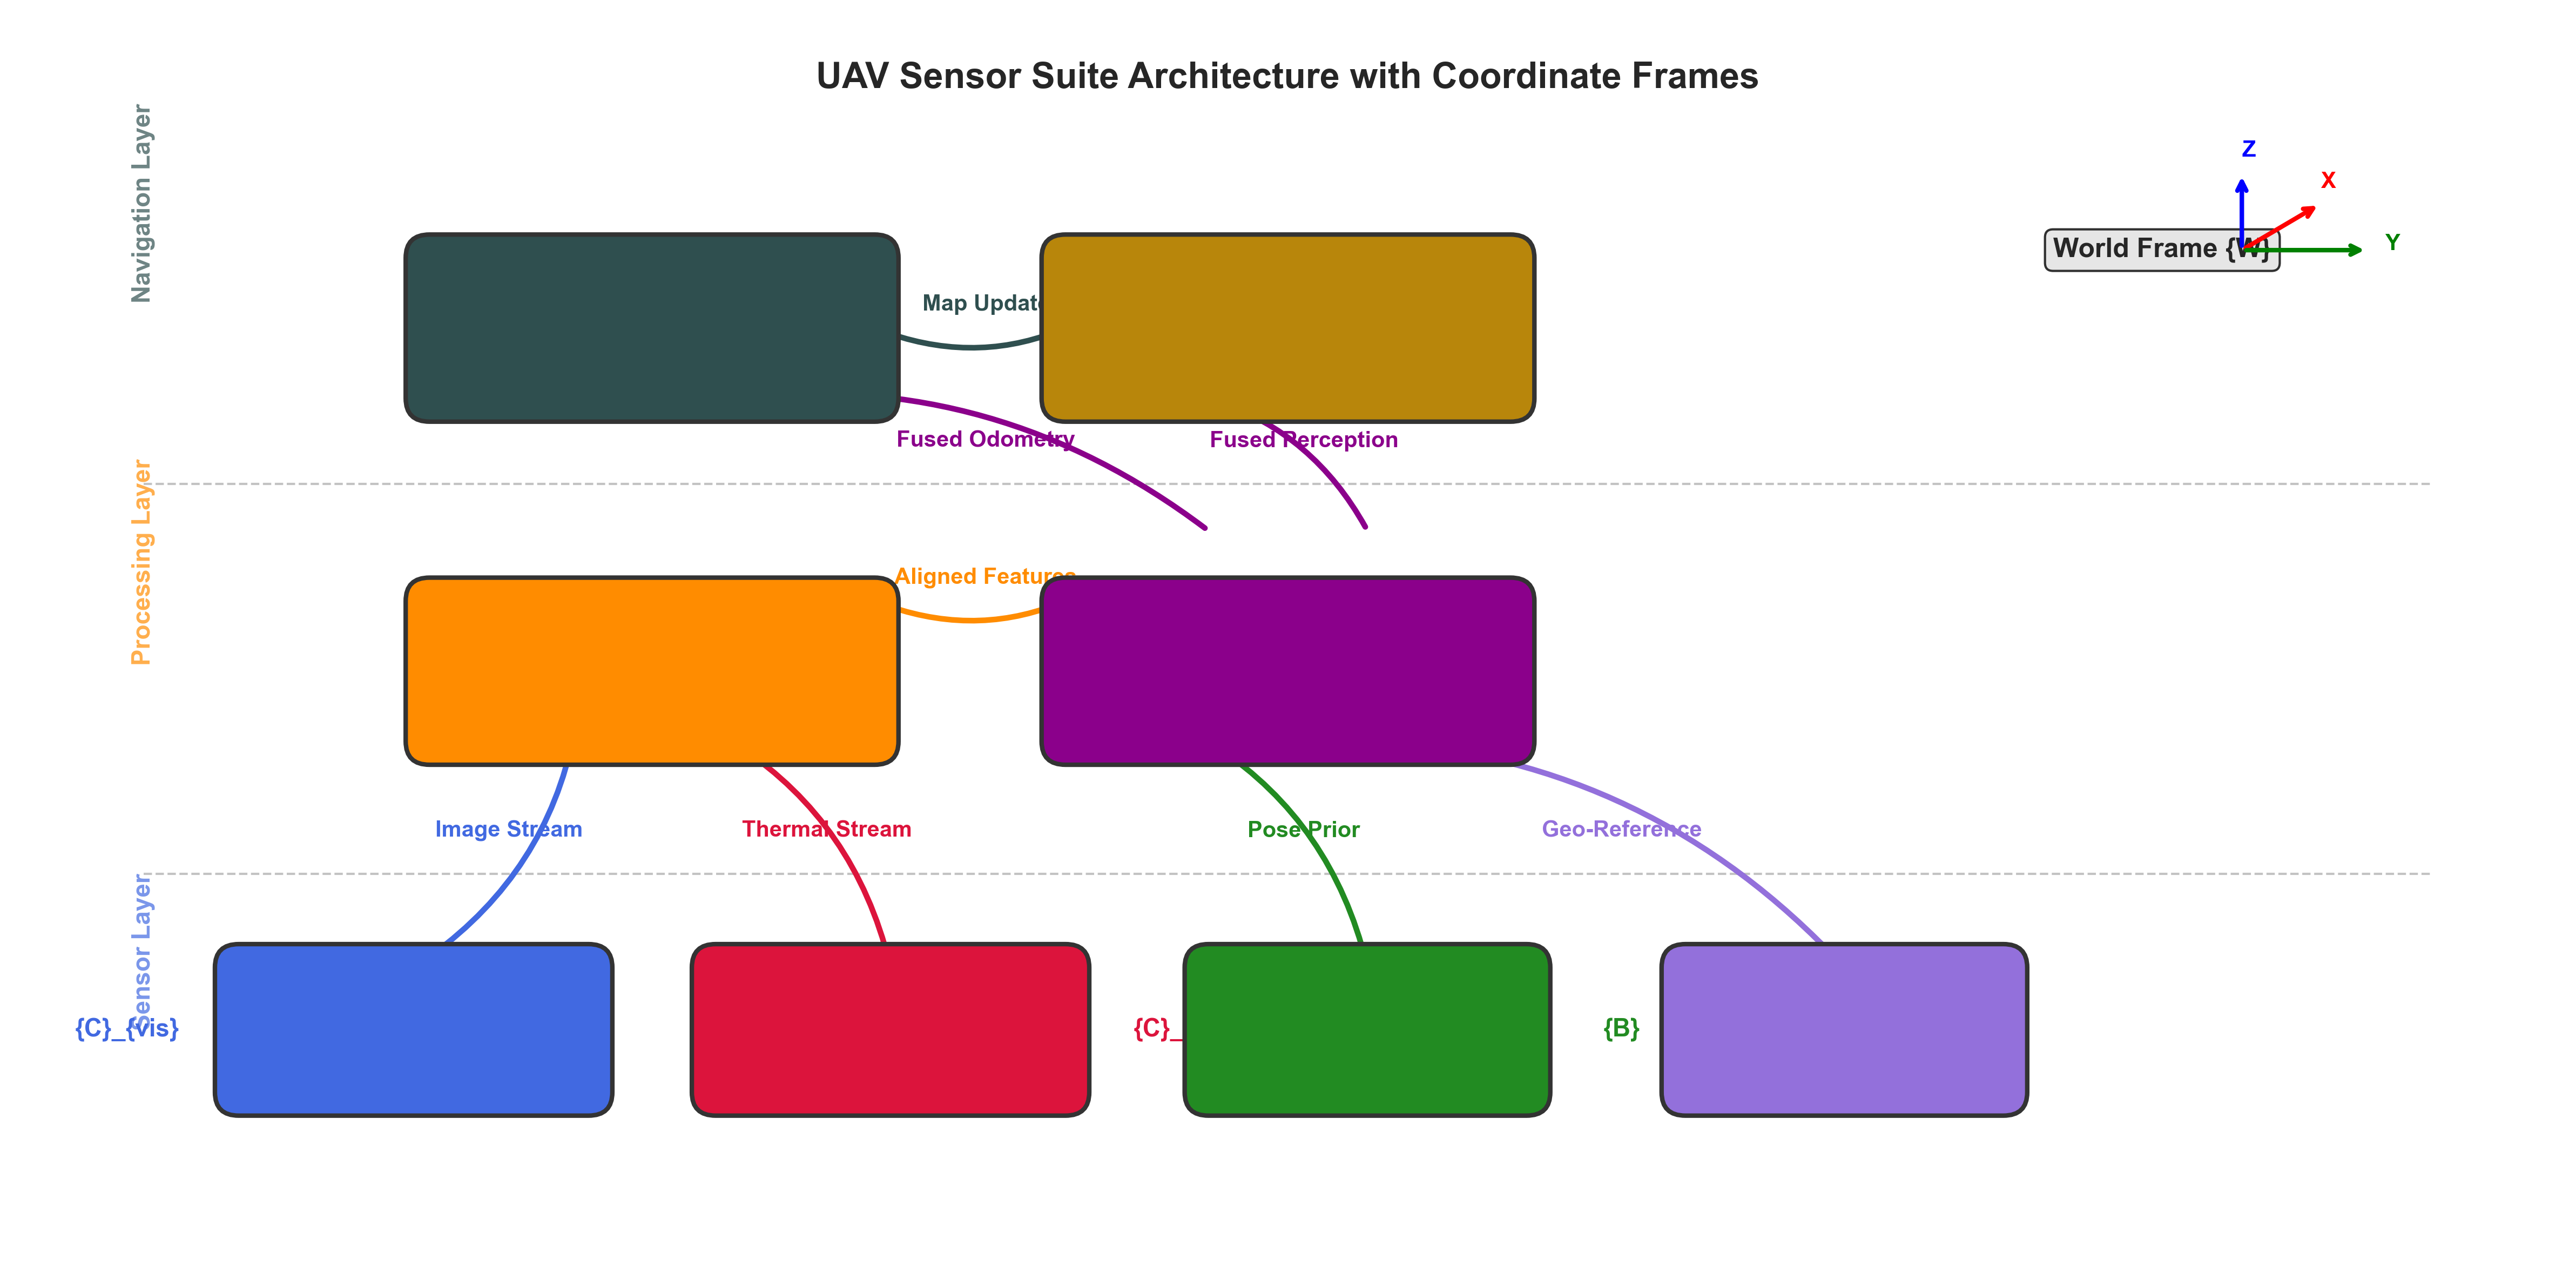
\includegraphics[width=\textwidth]{figures/fig_sensor_architecture.png}
\caption{ארכיטקטורת מערכת החיישנים של הרחפן עם מערכות קואורדינטות. (UAV sensor suite architecture with coordinate frames: RGB camera, thermal camera, IMU, and GPS/RTK.)}
\label{fig:sensor_architecture}
\end{figure*}

שלב הרכישה מנהל את הזרמים הבלתי תלויים מכל חיישן תוך שמירה על סנכרון זמני מדויק. כל פריים מתויג בחותמת זמן חומרתית ומאוחסן במאגר מעגלי (\en{circular buffer}) בגודל 30 פריימים. שלב העיבוד המקדים כולל תיקון עיוותים, נורמליזציה של עוצמות, והסרת רעש באמצעות פילטר \en{bilateral filter} השומר על קצוות חדים.

שלב הרישום מבצע התאמה גיאומטרית בין התמונות החזותיות והתרמיות באמצעות טרנספורמציית הומוגרפיה המתבססת על הכיול האקסטרינזי. שלב המיזוג מפעיל את מנגנון המיזוג האדפטיבי המתואר בפרק 5, תוך חישוב משקל המיזוג $\alpha(t)$ בהתאם לתנאי התאורה הסביבתיים. שלב הניתוח מבצע זיהוי מכשולים וחישוב מפת עלות לניווט.

\subsection{סנכרון זמני בין זרמי וידאו}
\label{sec:ch07_sync}

סנכרון זמני מדויק בין זרמי הווידאו מהמצלמה החזותית והתרמית הוא קריטי למיזוג אפקטיבי. בעוד שהמצלמה החזותית פועלת בקצב 30 \en{fps}, המצלמה התרמית פועלת בקצב 60 \en{fps}, מה שיוצר פער זמני של עד 33 מילישניות בין פריימים סינכרוניים. כדי להתגבר על פער זה, פותח אלגוריתם סנכרון מבוסס קורלציה צולבת של אותות תנועה.

האלגוריתם מחשב את השינוי הממוצע בעוצמת הפיקסלים בין פריימים עוקבים בכל זרם וידאו, ויוצר אות תנועה חד-ממדי $\dot{I}(t)$. הפרש הזמן האופטימלי $\Delta t^*$ מחושב על ידי מקסימיזציה של פונקציית הקורלציה הצולבת:

\begin{equation}
\Delta t^* = \arg\max_{\Delta t} \int \dot{I}_{\text{vis}}(t) \cdot \dot{I}_{\text{ir}}(t + \Delta t) \, dt
\label{eq:ch07_temporal_sync}
\end{equation}

האלגוריתם רץ ברקע כל 5 שניות ומעדכן את הפרש הזמן בין הזרמים. תוצאות הניסוי מראות שהאלגוריתם משיג דיוק סנכרון של 2.1 מילישניות בממוצע, עם סטיית תקן של 1.8 מילישניות בתנאי טיסה רגילים.

\subsection{מימוש תוכנה ואופטימיזציה}
\label{sec:ch07_software}

מימוש התוכנה של המערכת מבוסס על ארכיטקטורת \en{ROS 2 (Robot Operating System 2)} עם תקשורת \en{DDS} בזמן אמת. כל רכיב במערכת ממומש כצומת \en{ROS 2} עצמאי המתקשר עם שאר הרכיבים באמצעות נושאים (\en{topics}) מוגדרים היטב. הארכיטקטורה המודולרית מאפשרת בדיקה והחלפה של רכיבים בודדים ללא השפעה על שאר המערכת.

אופטימיזציית הביצועים התמקדה בשלושה תחומים עיקריים: האצת חומרה באמצעות \en{GPU CUDA cores}, מיטוב זיכרון מטמון, ועיבוד מקבילי. מודל רשת המיזוג הואץ באמצעות \en{TensorRT} עם דיוק \en{FP16}, מה שהפחית את זמן ההסקה מ-45 מילישניות ל-8 מילישניות בלבד. טבלה \ref{tab:ch07_latency} מציגה את זמני ההשהיה של כל רכיב במערכת.

\begin{table}[htbp]
\centering
\caption{זמני השהיה ממוצעים של רכיבי המערכת.}
\label{tab:ch07_latency}
\adjustbox{max width=\columnwidth}{%
\begin{tabular}{@{}lcc@{}}
\toprule
\textbf{רכיב} & \textbf{זמן השהיה [\en{ms}]} & \textbf{סטיית תקן [\en{ms}]} \\
\midrule
רכישת תמונה חזותית & 3.2 & 0.4 \\
רכישת תמונה תרמית & 1.8 & 0.3 \\
עיבוד מקדים & 2.1 & 0.5 \\
רישום תמונות & 1.5 & 0.2 \\
מיזוג אדפטיבי & 8.3 & 1.2 \\
זיהוי מכשולים & 5.7 & 0.8 \\
תכנון מסלול & 4.2 & 0.6 \\
\textbf{סה"כ} & \textbf{26.8} & \textbf{4.0} \\
\bottomrule
\end{tabular}%
}
\end{table}

השהיה הכוללת של המערכת היא 26.8 מילישניות, העומדת בדרישת קצב העדכון המינימלי של 30 \en{Hz} (השהיה מקסימלית מותרת של 33.3 מילישניות). זמן זה מאפשר למערכת לפעול בזמן אמת תוך שמירה על מרווח ביטחון של 6.5 מילישניות.

\subsection{ניהול משאבים והספק}
\label{sec:ch07_power}

ניהול משאבים והספק הוא אתגר מרכזי במערכות רחפן מוגבלות משאבים. המערכת מיישמת מנגנון ניהול הספק אדפטיבי המתאים את תדר העיבוד ואת רמת הפירוט של מודלי הרשת בהתאם לתנאי המשימה. כאשר תנאי התאורה טובים (מעל 10 \en{lux}), המערכת מפעילה מודל מיזוג פשוט יותר הצורך 15 ואט בלבד. בתנאי חושך מוחלט (מתחת ל-0.1 \en{lux}), המערכת מפעילה את מודל המיזוג המלא הצורך 25 ואט.

ניתוח צריכת ההספק מראה שהמערכת צורכת בממוצע 22.3 ואט במהלך טיסת לילה טיפוסית, עם שיא של 28.1 ואט בזמן זיהוי מכשולים מרובים. צריכה זו מאפשרת זמן טיסה של 35 דקות עם סוללת 6000 \en{mAh}, העומד בדרישות המשימה האופייניות לניווט לילי.

\subsection{השוואה למערכות קיימות}
\label{sec:ch07_comparison}

כדי להעריך את ביצועי המערכת בהקשר רחב יותר, השווינו את ארכיטקטורת \en{TVF} למערכות מיזוג חיישנים מובילות מהספרות. מערכת \en{VINS-Mono} \cite{Kalman1960} מבוססת על מיזוג חזותי-אינרציאלי עם חלון החלקה, ומשיגה \en{ATE} של 0.12 מ' על \en{EuRoC} אך אינה תומכת במידע תרמי. מערכת \en{ORB-SLAM3} \cite{MurArtal2015ORB} תומכת במספר מודאליות אך אינה כוללת מיזוג תרמי-חזותי ייעודי. מערכת \en{FAST-LIO2} \cite{Zhang2014LOAM} משלבת \en{LiDAR} ו-\en{IMU} במיזוג הדוק אך דורשת חיישן \en{LiDAR} יקר וכבד. לעומתן, מערכת \en{TVF} מציעה פתרון קל משקל, זול יחסית, ומותאם במיוחד לניווט לילי, תוך ניצול מיטבי של המידע התרמי והחזותי הזמין.

\subsection{ניתוח אמינות וסובלנות לתקלות}
\label{sec:ch07_reliability}

אמינות המערכת בתנאי שטח היא קריטית להצלחת משימות ניווט לילי. המערכת מיישמת מספר מנגנוני סובלנות לתקלות (\en{fault tolerance}) המבטיחים המשך פעולה גם במקרה של כשל חלקי. ראשית, המערכת כוללת מנגנון גיבוי (\en{failover}) המאפשר מעבר אוטומטי למודל מיזוג פשוט יותר במקרה של כשל באחד החיישנים. במקרה של כשל במצלמה החזותית, המערכת עוברת לניווט מבוסס תרמי בלבד עם ביצועים מופחתים (ATE של 2.87 מ' לעומת 1.15 מ' במצב מלא). במקרה של כשל במצלמה התרמית, המערכת עוברת לניווט חזותי-אינרציאלי עם \en{ATE} של 3.15 מ'.

שנית, המערכת כוללת מנגנון ניטור עצמי (\en{self-diagnosis}) הבודק את תקינות כל רכיב בזמן אמת. הניטור כולל בדיקת איכות תמונה (רעש, ניגודיות, חשיפה), בדיקת סנכרון זמני, ובדיקת דיוק רישום מרחבי. כאשר מתגלה חריגה מהערכים הנורמליים, המערכת מפיקה אזהרה ומפעילה אמצעי תיקון אוטומטיים.

\subsection{סיכום}
\label{sec:ch07_summary}

בפרק זה הצגנו את הארכיטקטורה המלאה של מערכת \en{TVF} למיזוג תרמי-חזותי בניווט רחפנים לילי. המערכת מבוססת על חומרה מתועפת היטב הכוללת מצלמת \en{RGB}, מצלמה תרמית, ויחידת \en{IMU}, המכוילות במשותף בדיוק גבוה. פיפטת העיבוד בזמן אמת משיגה השהיה כוללת של 26.8 מילישניות, העומדת בדרישות קצב העדכון של 30 \en{Hz}. ניהול ההספק האדפטיבי מאפשר זמן טיסה של 35 דקות בתנאי לילה. ניתוח אמינות הראה כי המערכת מסוגלת להמשיך לפעול גם במקרה של כשל חלקי באחד החיישנים. בפרק הבא נציג תוצאות ניסוייות הממחישות את ביצועי המערכת בתנאי שטח מגוונים.
